In this chapter, we present results from the expert review of the \gls{cci} and our psychometric analysis of students' responses to the \gls{cci}. To help the reader interpret our findings, we compare our results with three \glspl{cilabel} evaluated with the same techniques. These \glspl{cilabel} are the Concept Assessment Tool for Statics (27 questions and 1,372 students), the Statistics Concept Inventory (38 questions and 402 students), and the Dynamics Concept Inventory (29 questions and 5,966 students) \cite{jorian}. We chose these \glspl{cilabel} because they are the few technical \glspl{cilabel} that analyzed the \glspl{cilabel} using similar techniques. 

\section{Expert Panel}


The expert panel consisted of 12 experts in cybersecurity or a related field. These experts reviewed each of the individual items and rated them on a scale of Accept, Accept with Minor Revisions, Accept with Major Revisions, and Reject. The results of this review process can be seen in Figure \ref{fig:accept_rej}. Although 32 items were reviewed, the figure presents the results for the 24 items in the current CCI. The items selected for the \gls{cci} were reviewed positively receiving a vast majority of Accept and Accept with Minor Revisions.

Additionally, experts left comments for each item which we used to revise the items that received Reject ratings. As an example, we show how we used expert reviews to revise item Q4. Q4 covered a potential SQL injection vulnerability and the means of defending against it. The initial wording of the Q4 scenario is below.

\begin{quotation}
\noindent{\textbf{Scenario A3} When a user Mike O'Brien registered a new account for an online shopping site, he was required to provide his username, address, first and last name, and a password. Immediately after Mike submitted his request, you---as the security engineer---receive a database input error message in the logs.}
\end{quotation}


Experts commented that this wording is imprecise because an error in the logs is not ``received" but rather written into the log on the server. The word ``received" implies the error was noticeable and could lead students to infer that the error came from the client-side. The item was modified to replace ``receive a database input error" with ``observe a database input error." The change makes it clear that the user input did not cause an alert and that the message was logged on the server-side. The clarification will lead students away from client-side solutions such as ``more thoroughly test the software before deploying it" and toward server-side solutions such as the correct response, ``sanitize input at the server side." The expert review process strengthened the clarity which is critical to measuring a student's conceptual knowledge.

\iflong
\begin{figure}[!htbp]
    \begin{center}
    \advance\leftskip-3cm
    \advance\rightskip-3cm
    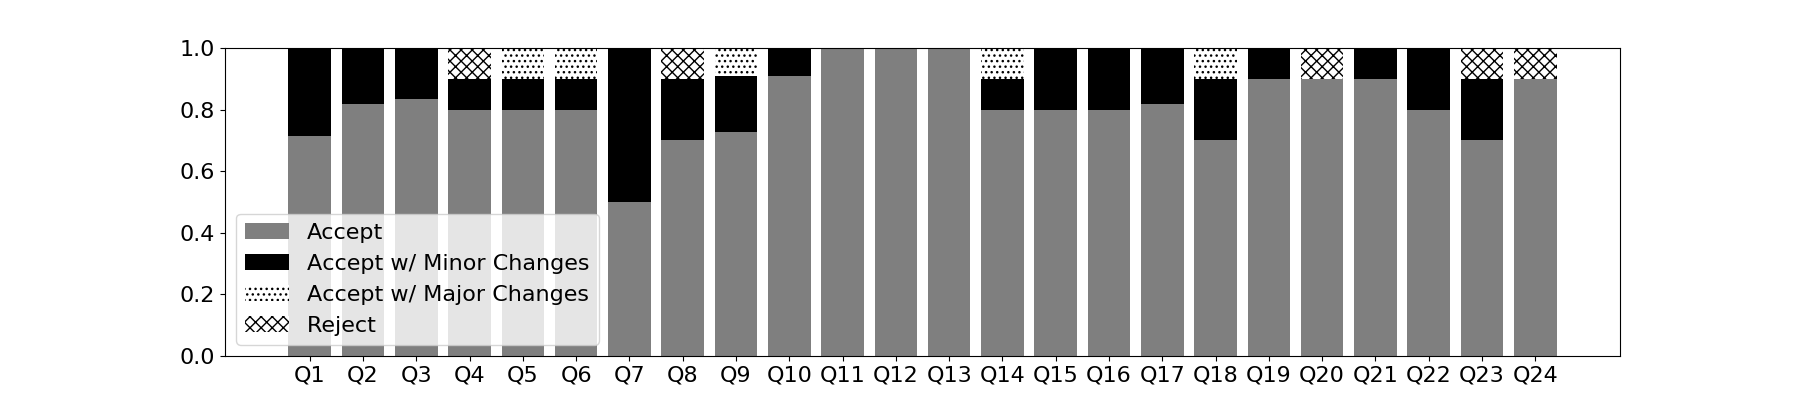
\includegraphics[scale=.4]{images/bar.png}
    \caption{Expert Response to Items}
    \label{fig:accept_rej}
\end{center}
\end{figure}
\fi

\ifshort
\begin{figure}[!htbp]
    \begin{center}
    \advance\leftskip-3cm
    \advance\rightskip-3cm
    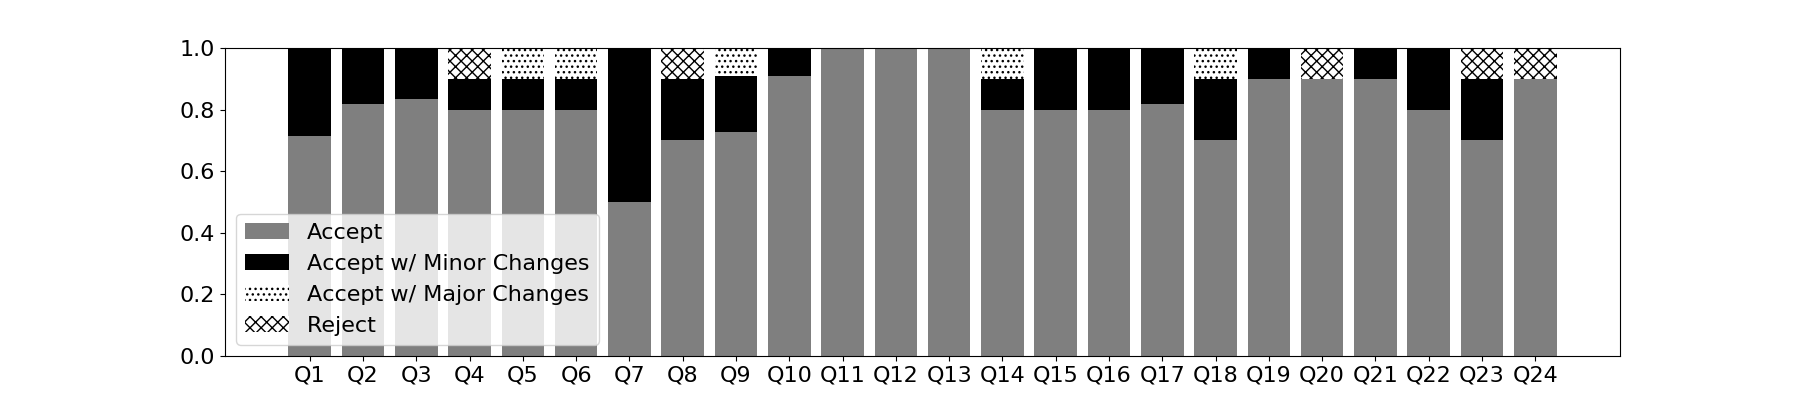
\includegraphics[scale=.3]{images/bar.png}
    \caption{Expert Response to Items}
    \label{fig:accept_rej}
\end{center}
\end{figure}
\fi

\FloatBarrier
\section{Reliability and Standard Error}

Cronbach's $\alpha$ is a measure of the reliability of the instrument. The Cronbach's $\alpha$ of the \gls{cci} in this pilot test is 0.78 which is close to Jorian et al.'s recommendation for good reliability of 0.80 and above Panayiotis's minimum recommendation of 0.70. The reliability of the \gls{cci} is similar to other \glspl{cilabel} as seen in Table \ref{tab:compare}. The reliability of the \gls{cci} suggests that it is sufficiently reliable to be a valid \gls{cilabel}.   


The standard error of measurement defines a confidence interval for each student's true score. The standard measurement error of the \gls{cci} was 2.13 for this pilot test. A 2.13 standard error implies the 68\% confidence interval for a student’s true score, given that a mean observed score of 8.61 points is from 6.48 to 10.74. 

\FloatBarrier

\begin{table*}[!htbp]   
\caption{Comparison with Other Instruments: Concept Assessment Tool for Statics, Statistics Concept Inventory, Dynamics Concept Inventory \cite{jorian}}   
\centering   
\begin{tabular}[width=\textwidth]{ccccc}   
    \toprule
    \textbf{Measurement} & \textbf{\gls{cci}} & \textbf{Statics} & \textbf{Statistics} & \textbf{Dynamics} \\
    \textit{Cronbach's $\alpha$} & 0.78 & 0.84 & 0.64 & 0.74\\   
    \textit{Minimum Difficulty Value} & 0.10 & 0.16 & 0.03 & 0.06 \\   
    \textit{Maximum Difficulty Value} & 0.66 & 0.78 & 0.87 & 0.91 \\   
    \textit{Minimum Discrimination Value} & 0.16 & 0.18 & -0.13 & 0.01\\
    \textit{Maximum Discrimination Value} & 0.47 & 0.65 & -0.57 & 0.56\\   
    \bottomrule   
\end{tabular}   
\label{tab:compare}   
\end{table*}  

\begin{table}[!htbp]
\caption{Instrument Statistics}
\centering
\begin{tabular}{cc}
    \toprule
    \textit{Cronbach's $\alpha$} & 0.78 \\
    \textit{Standard Error of Measurement} & 2.13 \\
    \textit{Mean (Out of 25)} & 8.61\\
    \textit{Standard Deviation} & 4.58\\
    \bottomrule
\end{tabular}
\label{tab:overall}
\end{table}


Cronbach's $\alpha$ can be used as a coarse evaluation of the quality of an item. Each item should increase the quality of the instrument, and excluding that item should decrease the overall reliability. Table \ref{tab:table_cronbach_exclusion} shows the results of the Cronbach calculation with each item excluded. Ideally, every item would be below the original Cronbach $\alpha$ indicating that each item increases the overall reliability. There are no items that decrease the overall reliability and consequently need to be removed.

\iffalse
\iflong
\begin{figure}[ht]
    \begin{center}
    \advance\leftskip-.25cm
    \advance\rightskip-.25cm
    \includegraphics[scale=.5]{images/Cronobach's.png}
    \caption{Cronbach's $\alpha$ with Items Excluded}
    \label{fig:cron}
\end{center}
\end{figure}
\fi
\fi
\input{tex/alpha_table.tex}

\FloatBarrier
\section{Difficulty and Discrimination}

The difficulty of an item is the fraction of students with the correct response. If an item is too hard, the item is separating only strong students from strong students. If an item is too easy, it cannot differentiate any students. The acceptable range of difficulty is between 0.20 and 0.80. The difficulty of each item can be seen in Figure \ref{fig:dif_disc} and Table \ref{tab:diff_v_discrimination}. The range of difficulty for the \gls{cci} is 0.10 to 0.66. When compared to the other instruments the \gls{cci} seen in Table \ref{tab:compare} it is too difficult and will have less discriminatory power. The \gls{cci} instrument overall is too difficult as evidenced by 21 out of 25 items having difficulty below 0.50 and 5 items falling outside the minimum acceptable difficulty. 

The discrimination of an item indicates the amount of information an item gives about the overall performance of the student. High discrimination indicates that a student's performance on a given item is highly correlated to overall performance. The acceptable range of discrimination is anything above 0.20.  Figure \ref{fig:dif_disc} shows the discrimination of each item. The range of discrimination is 0.16 to 0.47. The discrimination range is not as high as other \glspl{cilabel} seen in Table \ref{tab:compare}, but the bottom of the range is much higher than the Statistics Concept Inventory and Dynamics Concept Inventory. The other \glspl{cilabel} had one, ten, and five items fall below the 0.20, while the \gls{cci} had three items below 0.20. Most of the items being above the minimum value is encouraging indicator the assessment is valid.   

\iffalse
\iflong
The correlation coefficient can be calculated for each item to quantify how similar the item fits in with the rest of the items. The correlation for each item can be seen in Figure \ref{fig:correlation}. 


\begin{figure}[!hbp]
    \begin{center}
    \advance\leftskip-3cm
    \advance\rightskip-3cm
    \includegraphics[scale=.45]{images/correlation.png}
    \caption{Correlation}
    \label{fig:correlation}
\end{center}
\end{figure}
\fi
\fi

\begin{table}[!htbp]
\caption{Difficulty and Discrimination of Each Item}
\centering
\scalebox{.7}{
\begin{tabular}{cccccc}
    \toprule
    Item & Discrimination & Difficulty & Item & Discrimination & Difficulty\\
    \midrule
    \textit{Q1} & 0.22 & 0.24 & \textit{Q14} & 0.32 & 0.25 \\
    \textit{Q2} & 0.32 & 0.33 & \textit{Q15} & 0.25 & 0.10 \\
    \textit{Q3} & 0.16 & 0.26 & \textit{Q16} & 0.35 & 0.59 \\
    \textit{Q4} & 0.46 & 0.52 & \textit{Q17} & 0.35 & 0.52 \\
    \textit{Q5} & 0.35 & 0.18 & \textit{Q18} & 0.19 & 0.31 \\
    \textit{Q6} & 0.23 & 0.22 & \textit{Q19} & 0.27 & 0.28 \\
    \textit{Q7} & 0.30 & 0.66 & \textit{Q20} & 0.22 & 0.14 \\
    \textit{Q8} & 0.21 & 0.19 & \textit{Q21} & 0.23 & 0.44 \\
    \textit{Q9} & 0.33 & 0.61 & \textit{Q22} & 0.47 & 0.34 \\
    \textit{Q10} & 0.19 & 0.40 & \textit{Q23} & 0.38 & 0.49 \\
    \textit{Q11} & 0.34 & 0.36 & \textit{Q24} & 0.30 & 0.40 \\
    \textit{Q12} & 0.36 & 0.24 & \textit{Q25} & 0.24 & 0.14 \\
    \textit{Q13} & 0.21 & 0.28 & \textit{} &  &\\
    \bottomrule
\end{tabular}
}
\label{tab:diff_v_discrimination}
\end{table}




\begin{figure}[ht]
    \begin{center}
    \advance\leftskip-.25cm
    \advance\rightskip-.25cm
    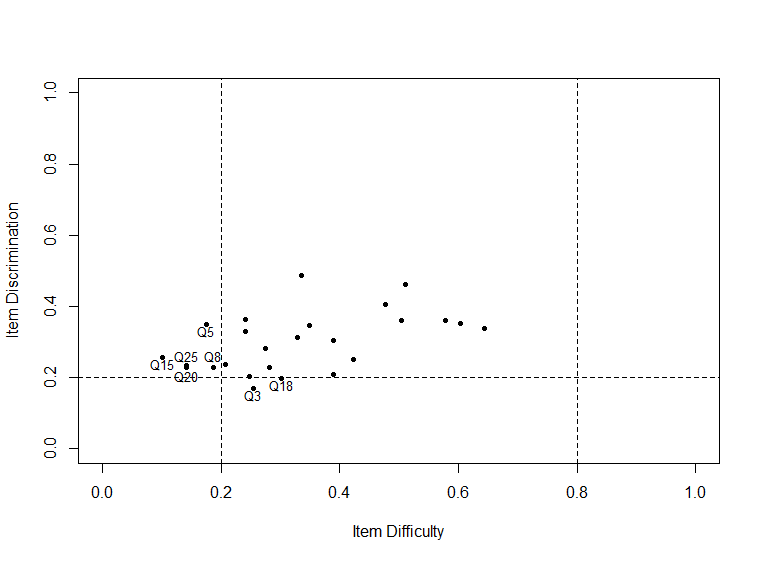
\includegraphics[scale=.45]{images/new_graph.png}
    \caption{Difficulty vs. Discrimination}
    \label{fig:dif_disc}
\end{center}
\end{figure}



\FloatBarrier
\section{Concept Subtests}
The \gls{cci} consists of five concepts: \gls{v}, \gls{c}, \gls{d}, \gls{g}, and \gls{t}. Each item assesses one of these concepts. The individual items within a concept can be grouped and the Cronbach's $\alpha$ calculated to evaluate the reliability of that concept subtest. The $\alpha$'s of the concept subtests are seen in Table \ref{tab:alpha_concept}. When evaluating the concepts, it is notable that all of the values are significantly less than 0.70 which is considered the minimum acceptable value for a reliable instrument \cite{panayiotis}. These findings suggest that the subtests should not be used as evaluations of students' knowledge of the specific concepts. 

%Specifically, \gls{v} has a poor $\alpha$ of 0.236 indicating that the evaluation of that concept through this \gls{cci} is not practical. 

\begin{table}[!htbp]
\caption{Cronbach's $\alpha$ by Concept}
\centering
\scalebox{.8}{
\begin{tabular}{ccc}
    \toprule
    Concept & Cronbach's $\alpha$ & Items Included \\
    \midrule
    \textit{V} & 0.22 & Q1, Q3, Q11, Q17, Q21\\
    \textit{C} & 0.45 & Q2, Q5, Q14, Q18, Q24\\
    \textit{D} & 0.47 & Q4, Q6, Q13, Q19, Q23\\
    \textit{G} & 0.36 & Q8, Q9, Q10, Q22, Q25\\
    \textit{T} & 0.50 & Q7, Q12, Q15, Q16, Q20\\
    \bottomrule
\end{tabular}
}
\label{tab:alpha_concept}
\end{table}


\iflong

The correlation between items in the subtests can be expressed with a correlation matrix. The correlation matrix is the correlation coefficient of each item with every other item. A heat map of the correlation matrix can be seen in Figure \ref{fig:alignment}. The square regions enclose the items in a specific concept subtest. Items within the same concept subtest should be expected to correlate strongly with each other compared to items outside their subtest. We do not see these types of stronger and weaker correlations. 

\begin{figure}[!hbp]
    \centering
    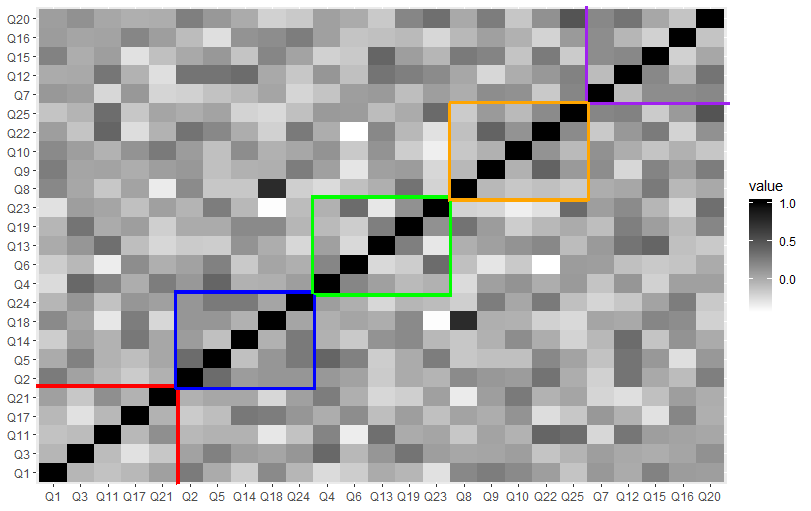
\includegraphics[scale=1.4]{images/heat_map_top_quarter.png}
    \begin{minipage}{0.65\linewidth}
    \tiny
    \emph{
    V: Red,
    C: Blue,
    D: Green,
    G: Orange,
    T: Purple
    }
    \end{minipage}
    \caption{Concept Alignment of Top Quarile}
    \label{fig:alignment}
\end{figure}
\fi

\FloatBarrier
\section{Deeper Analysis of Specific Items}

The psychometric analysis of the \gls{cci} revealed that the instrument has too many difficult items. To inform future revisions of the \gls{cci}, we are analyzing the distractor distribution and distractor discrimination to understand why some items are so difficult. We present an example of this for one of these items, Q15, which had a low difficulty of 0.10 and relatively low discrimination of 0.25 in the pilot trial. We compare Q15 to a stronger item, Q4, which had a good difficulty of 0.52 and discrimination of 0.46 in the pilot trial. 

The distractor analysis shows the proportion of the students' responses in each tertile. The distractor analysis for both Q15 and Q4 can be seen in Table \ref{tab:table_distract}. In Q4, which has a good distribution, the percentage of students getting the correct answer increases from the bottom tertile to the top, and the top tertile generally answers the question correctly. For Q15, although the percentage of students selecting the correct answer increases from the bottom tertile to the top, there is little difference between the top and middle tertiles. Additionally, the top-tertile students answer Q15 correctly 18\% of the time and instead select distractor A 59\% of the time. The preference for option A among the top tertile is causing the item to be too difficult.

\begin{table}[!htbp]
\caption{Distractor Distribution (Asterisk Identifies Correct Alternative)}
\hspace{\fill}
\begin{subtable}[!htbp]{0.45\textwidth}
\flushright
\scalebox{.9}{
\begin{tabular}[!htbp]{c c c c}
\toprule
\textbf{Q4} &  &  &  \\
\midrule
\textit{Response} & \textit{Lower} & \textit{Middle} & \textit{Upper} \\
A & 0.02 & 0 & 0.03 \\
*B & 0.28 & 0.62 & 0.85 \\
C & 0.11 & 0 & 0.26 \\
D & 0.37 & 0.14 & 0 \\
E & .22 & 0.24 & 0.10 \\
blank & 0.02 & 0 & 0 \\
\bottomrule
\end{tabular}
}
\end{subtable}
\hspace{\fill}
\begin{subtable}[!htbp]{0.45\textwidth}
\flushright
\scalebox{.9}{
\begin{tabular}[!htbp]{c c c c}
\toprule
\textbf{Q15} &  &  &  \\
\midrule
\textit{Response} & \textit{Lower} & \textit{Middle} & \textit{Upper} \\
A & 0.22 & 0.36 & 0.59 \\
B & 0.39 & 0.26 & 0.08 \\
C & 0.15 & 0.17 & 0.15 \\
D & 0.22 & 0.05 & 0 \\
*E & 0 & 0.17 & 0.18 \\
blank & 0.02 & 0 & 0 \\
\bottomrule
\end{tabular}
}
\end{subtable}
\label{tab:table_distract}
\end{table}



\iffalse
\hspace{\fill}
\begin{subtable}[!htbp]{0.45\textwidth}
\flushright
\scalebox{.9}{
\begin{tabular}[!htbp]{c c c c}
\toprule
\textbf{Q22} &  &  &  \\
\midrule
\textit{Response} & \textit{Lower} & \textit{Middle} & \textit{Upper} \\
A & 0.06 & 0.02 & 0\\
B & 0.13 & 0.071 & 0.02\\
blank & 0.04 & 0 & 0\\
C & 0.50 & 0.60 & 0.23\\
*D & 0.15 & 0.29 & 0.74\\
E & 0.13 & 0.02 & 0\\
\bottomrule
\end{tabular}
}
\label{tab:table1_d}
\end{subtable}


\begin{subtable}[!htbp]{0.5\textwidth}
\flushright
\scalebox{.9}{
\begin{tabular}[!htbp]{c c c c}
\toprule
\textbf{Q3} &  &  &   \\
\midrule
\textit{Response} & \textit{Lower} & \textit{Middle} & \textit{Upper} \\
A & 0.37 & 0.429 & 0.256 \\
B & 0.13 & 0.238 & 0.128 \\
C & 0.204 & 0.024 & 0.103 \\
*D & 0.204 & 0.214 & 0.436 \\
E & 0.093 & 0.095 & 0.077 \\
blank & 0 & 0 & 0 \\
\bottomrule
\end{tabular}
}
%\caption{\footnotesize Question 3 Distractors}
\label{tab:table1_a}
\end{subtable}
\begin{table}[!htbp]
\caption{Distractor Distribution}
\begin{subtable}[!htbp]{0.5\textwidth}
\flushright
\scalebox{.66}{
\begin{tabular}[!htbp]{c c c c}
\toprule
\textbf{Q3} &  &  &   \\
\midrule
\textit{Response} & \textit{Lower} & \textit{Middle} & \textit{Upper} \\
A & 0.37 & 0.429 & 0.256 \\
B & 0.13 & 0.238 & 0.128 \\
C & 0.204 & 0.024 & 0.103 \\
*D & 0.204 & 0.214 & 0.436 \\
E & 0.093 & 0.095 & 0.077 \\
blank & 0 & 0 & 0 \\
\bottomrule
\end{tabular}
}
%\caption{\footnotesize Question 3 Distractors}
\label{tab:table1_a}
\end{subtable}
\hspace{\fill}
\begin{subtable}[!htbp]{0.5\textwidth}
\flushright
\scalebox{.66}{
\begin{tabular}[!htbp]{c c c c}
\toprule
\textbf{Q5} &  &  &   \\
\midrule
\textit{Response} & \textit{Lower} & \textit{Middle} & \textit{Upper} \\
A & 0.389 & 0.524 & 0.308 \\
B & 0.167 & 0.071 & 0.051 \\
C & 0.278 & 0.167 & 0.128 \\
D & 0.074 & 0.167 & 0.077 \\
*E & 0.093 & 0.071 & 0.436 \\
blank & 0 & 0 & 0 \\
\bottomrule
\end{tabular}
}
\label{tab:table1_b}
\end{subtable}
\hspace{\fill}
\begin{subtable}[!htbp]{0.5\textwidth}
\flushright
\scalebox{.66}{
\begin{tabular}[!htbp]{c c c c}
\toprule
\textbf{Q8} &  &  &  \\
\midrule
\textit{Response} & \textit{Lower} & \textit{Middle} & \textit{Upper} \\
A & 0.333 & 0.357 & 0.154 \\
B & 0.463 & 0.31 & 0.513 \\
*C & 0.074 & 0.238 & 0.333 \\
D & 0.074 & 0 & 0 \\
E & 0.056 & 0.095 & 0 \\
blank & 0 & 0 & 0 \\
\bottomrule
\end{tabular}
}
\label{tab:table1_c}
\end{subtable}
\hspace{\fill}
\begin{subtable}[!htbp]{0.5\textwidth}
\flushright
\scalebox{.66}{
\begin{tabular}[!htbp]{c c c c}
\toprule
\textbf{Q15} &  &  &  \\
\midrule
\textit{Response} & \textit{Lower} & \textit{Middle} & \textit{Upper} \\
A & 0.222 & 0.357 & 0.59 \\
B & 0.389 & 0.262 & 0.077 \\
C & 0.148 & 0.167 & 0.154 \\
D & 0.222 & 0.048 & 0 \\
*E & 0 & 0.167 & 0.179 \\
blank & 0.019 & 0 & 0 \\
\bottomrule
\end{tabular}
}
\label{tab:table1_d}
\end{subtable}
\hspace{\fill}
\begin{subtable}[!htbp]{0.5\textwidth}
\flushright
\scalebox{.66}{
\begin{tabular}[!htbp]{c c c c}
\toprule
\textbf{Q20} &  &  &  \\
\midrule
\textit{Response} & \textit{Lower} & \textit{Middle} & \textit{Upper} \\
A & 0.222 & 0.143 & 0 \\
*B & 0.074 & 0.167 & 0.231 \\
C & 0.333 & 0.262 & 0.308 \\
D & 0.222 & 0.119 & 0.051 \\
E & 0.093 & 0.31 & 0.41 \\
blank & 0.056 & 0 & 0 \\
\bottomrule
\end{tabular}
}
\label{tab:table1_e}
\end{subtable}
\hspace{\fill}
\begin{subtable}[!htbp]{0.5\textwidth}
\flushright
\scalebox{.66}{
\begin{tabular}[!htbp]{c c c c}
\toprule
\textbf{Q25} &  &  &  \\
\midrule
\textit{Response} & \textit{Lower} & \textit{Middle} & \textit{Upper} \\
*A & 0.093 & 0.095 & 0.282 \\
B & 0.241 & 0.286 & 0.205 \\
C & 0.259 & 0.19 & 0.128 \\
D & 0.167 & 0.167 & 0.128 \\
E & 0.204 & 0.262 & 0.256 \\
blank & 0.037 & 0 & 0 \\
\bottomrule
\end{tabular}
}
\label{tab:table1_f}
\end{subtable}
\label{tab:table_distract}
\end{table}
\fi

 
 Table \ref{tab:table_distract_discrim} shows the distractor discrimination value for both Q4 and Q15. We expect the distractors to have negative discrimination values. Q4 has negative or zero distractor discrimination values for each distractor as well as a large positive discrimination value for the correct answer. Q15 does have a large positive discrimination for the correct answer and is even above the minimum acceptable value, but distractor A has a larger, positive discrimination value. This analysis reveals that for some reason the correct answer is not compelling to the strongest students, suggesting that the wording or structure of the answer choices may be to blame. We explore this assertion more in future work.

\begin{table}[!ht]
\caption{Distractor Discrimination Values (Asterisk Identifies Correct Alternative)}
\hspace{\fill}
\begin{subtable}[!htbp]{0.45\textwidth}
\flushright
\scalebox{1}{
\begin{tabular}[!htbp]{c c}
\toprule
\textbf{Q4} &  \\
\midrule
\textit{Distractor} & \textit{Discrimination} \\
A & 0 \\
*B & 0.46 \\
C & -0.14 \\
D & -0.26 \\
E & -0.04 \\
\bottomrule
\end{tabular}
}
\label{tab:table4_c}
\end{subtable}
\hspace{\fill}
\begin{subtable}[!htbp]{0.45\textwidth}
\flushright
\scalebox{1}{
\begin{tabular}[!htbp]{c c}
\toprule
\textbf{Q15} & \\
\midrule
\textit{Distractor} & \textit{Discrimination} \\
A & 0.35  \\
B & -0.19 \\
C & 0 \\
D & -0.26 \\
*E & 0.24  \\
\bottomrule
\end{tabular}
}
\label{tab:table4_d}
\end{subtable}
\label{tab:table_distract_discrim}
\end{table}



\iffalse

\hspace{\fill}
\begin{subtable}[!htbp]{0.45\textwidth}
\flushright
\scalebox{1}{
\begin{tabular}[!htbp]{c c}
\toprule
\textbf{Q22} & \\
\midrule
\textit{Distractor} & \textit{Discrimination} \\
A & -0.09 \\
B & -0.09 \\
C & -.08 \\
*D & 0.47 \\
E & -0.14 \\
\bottomrule
\end{tabular}
}
\label{tab:table4_d}
\end{subtable}
\begin{subtable}[!htbp]{0.5\textwidth}
\flushright
\scalebox{1}{
\begin{tabular}[!htbp]{c c}
\toprule
\textbf{Q3} &   \\
\midrule
\textit{Distractor} & \textit{Discrimination} \\
A & -0.0465  \\
B & 0.0618 \\
C & -0.152 \\
*D & 0.169\\
E & -0.028 \\
\bottomrule
\end{tabular}
}
%\caption{\footnotesize Question 3 Distractors}
\label{tab:table4_b}
\end{subtable}

\fi